\section{Materiales y métodos}\label{sec:metodos}
\subsection{Caso sintético y datos}
El caso es sintético y no representa una obra ni un levantamiento reales. Se adopta $Q_0=12.00\,\Qs$, $g=9.81\,\mathrm{m/s^2}$ y $z_J=100.00$ m. Los anchos de fondo son $b_0=4$ m (canal principal), $b_1=3$ m y $b_2=2$ m; la Tabla~\ref{tab:datos} reúne el resto. El canal principal no interviene en las ecuaciones 1D, pero sí en la geometría 2D. Se consideran cinco ángulos entre ejes: $30^\circ$, $45^\circ$, $60^\circ$, $90^\circ$ y $120^\circ$. El esquema isométrico del canal se muestra en la Figura~\ref{fig:esquema}. Los datos están en \path{datos/datos_entrada.json}.

\begin{table}[H]
\centering\small
\caption{Datos de entrada del caso nominal.}\label{tab:datos}
\begin{tabular}{lrr}
\toprule
Parámetro & Ramal 1 & Ramal 2\\\midrule
Ancho de fondo $b$ (m) & 3.00 & 2.00\\
Longitud $L$ (m) & 200 & 150\\
Rugosidad de Manning $n$ & 0.015 & 0.018\\
Pendiente de fondo $S$ (m/m) & 0.0008 & 0.0010\\
Calado de control $y_d$ (m) & 1.60 & 1.40\\
Cota de fondo en la unión $z_J$ (m) & 100.00 & 100.00\\
Coeficiente local $K$ & 0.20 & 0.20\\\bottomrule
\end{tabular}
\Fuente{Elaboración propia (caso sintético).}
\end{table}

\begin{figure}[H]
\centering
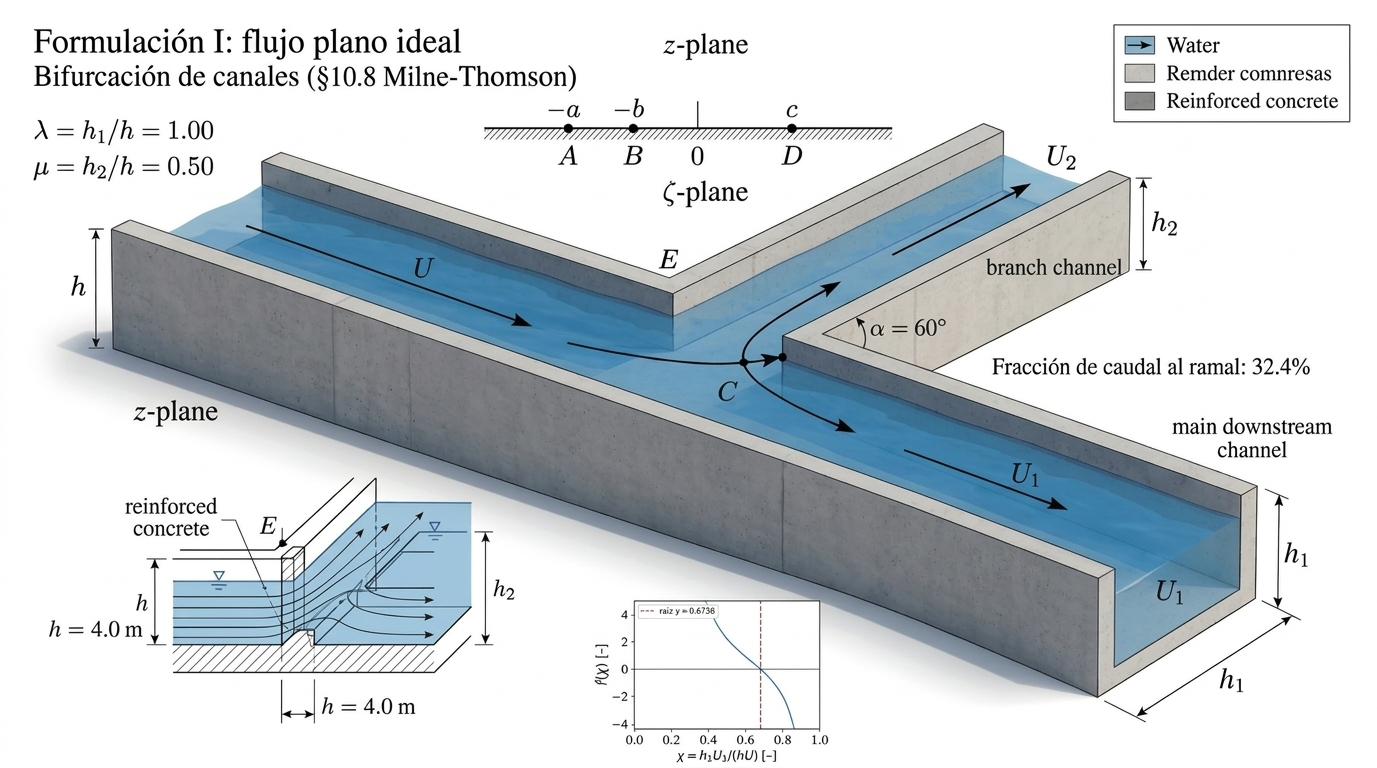
\includegraphics[width=0.82\linewidth,height=0.42\textheight,keepaspectratio]{2.png}
\caption{Esquema isométrico del canal bifurcado y nomenclatura. Ilustrativo, no a escala.}\label{fig:esquema}
\Fuente{Elaboración propia.}
\end{figure}

\subsection{Implementación numérica y reproducibilidad}
El código está en Python 3.13 con NumPy 2.5, pandas 3.0 y Matplotlib 3.11. La Formulación I se resuelve con Newton--Raphson sobre \eqref{eq:f1} para cada $\alpha$. La Formulación II usa Newton amortiguado con el jacobiano analítico \eqref{eq:sistema}, resolución del sistema lineal con \texttt{numpy.linalg.solve}, tolerancia $10^{-12}$ sobre $\|\mathbf F\|_\infty$, máximo de 50 iteraciones y retroceso hasta un factor mínimo de $10^{-4}$. El punto inicial reparte $Q_0$ según las conductancias de los ramales evaluadas con sus calados de control y coloca $H_J$ $0.05$ m sobre el mayor nivel terminal. El Monte Carlo usa 1500 realizaciones, desviaciones independientes y normales (caudal 5\pc, anchos 2\pc, Manning 10\pc, longitudes 2\pc, pendientes 5\pc, calados de control 0.04 m, $K$ 0.10 en valor absoluto) y la semilla fija \texttt{20261103}. Los resultados 1D se regeneran con \path{codigo/newton_bifurcacion.py}, que imprime las versiones de las bibliotecas y el historial de iteraciones.

\subsection{Pruebas de verificación del código}
Se aplican tres pruebas: (i) simetría analítica, con dos ramales idénticos el reparto debe ser $Q_0/2$ a cada lado; (ii) conservación de masa del caso nominal, $Q_1+Q_2-Q_0$; y (iii) contraste con una red de ocho canales publicada \citep[cap.~6]{chaudhry2008}. Además, las hojas de resultados 1D entregadas junto con el libro de HEC-RAS se contrastan con las soluciones recalculadas.

\subsection{Modelo bidimensional}\label{sec:hecras}
Las simulaciones usan los paquetes v3 del generador de geometría 2D, que reúnen los cambios derivados de las pruebas de verificación (Sección~\ref{sec:verif2d}); se ejecutaron en HEC-RAS 6.6/7.0 (unidades SI) por los tres integrantes del grupo, con la misma configuración para los cinco ángulos.
\begin{itemize}
\item \textbf{Ecuaciones:} SWE-EM (\emph{stricter momentum}), $\theta=1$, Courant adaptativo con máximo 1.0.
\item \textbf{Terreno y rugosidad:} raster de terreno y de Manning con celda de 0.05 m; $n=0.015$ en el canal principal y el ramal 1 y $n=0.018$ en el ramal 2. Canal de entrada de 50 m; las líneas de condición de borde se acortan 0.05 m por extremo y el fondo se abre 1.5 m aguas afuera de cada salida.
\item \textbf{Condiciones de borde:} hidrograma de entrada de 0.5 a $12\,\Qs$ en 600 s, mantenido hasta 7200 s; nivel fijo en las salidas (101.44 m en el ramal 1 y 101.25 m en el ramal 2), que equivale a los calados de control nominales de 1.60 y 1.40 m.
\item \textbf{Malla:} malla uniforme de 0.25 m para los cinco ángulos; en 30° y 120° se añadieron mallas de 0.50 y 0.125 m y regiones de refinamiento local en el nudo (0.125 y 0.0625 m sobre unos 90 m$^2$).
\item \textbf{Reparto:} $\varphi=Q_2/Q_0$ con los caudales de las líneas de borde de salida promediados en los últimos 600 s.
\end{itemize}
Una corrida se acepta si el error de volumen es menor que 0.5\pc, el cierre $|Q_1+Q_2-Q_0|/Q_0$ es menor que 1\pc y el caudal es estable entre los últimos 600 s y los 600 s previos (diferencia menor que 0.5\pc).

\subsection{Verificación en ramales rectos aislados}\label{sec:verif2d}
Antes de interpretar el reparto se simuló cada ramal por separado, recto, con su caudal nominal ($6.9405$ y $5.0595\,\Qs$) y su nivel de salida, y se comparó el perfil de la superficie con el remanso 1D integrado por Runge--Kutta de cuarto orden. La resistencia efectiva se calculó con \eqref{eq:neff}; el estimador devuelve $0.01500$ y $0.01795$ sobre los perfiles 1D, de modo que no tiene sesgo. Con celdas de 0.50, 0.25 y 0.125 m se obtuvo $n_\mathrm{eff}/n$ para los dos ramales. Después se probó una corrección lineal: ingresar $n/(n_\mathrm{eff}/n)$ medido a 0.25 m ($0.0174$ y $0.0212$) y comprobar que $n_\mathrm{eff}$ y el nivel recuperan los valores nominales, con tolerancia de $\pm0.01$ m.

\subsection{Conjunto exploratorio con SWE-ELM}
Un integrante ejecutó además un conjunto con SWE-ELM, celdas de 0.50, 0.25 y 0.125 m y los cinco ángulos, con un paquete anterior del generador. Los caudales se midieron en secciones transversales de los resultados. Se informa como exploratorio porque SWE-ELM no pasó la verificación en ramales diagonales estrechos y porque el paquete no incorpora las correcciones de la v3.

\subsection{Balance de masa}
El balance de volumen se tomó del resumen de cálculo de cada plan (\textit{Volume Accounting}; \citealt{hecmass}). El error relativo se define como $100\,(V_\mathrm{ent}-V_\mathrm{sal}-\Delta V_\mathrm{alm})/V_\mathrm{ent}$.
